\let\lesson\undefined
\newcommand{\lesson}{\phantomlesson{Bài 11.}}
\setcounter{section}{2}
\section{Bài tập trắc nghiệm}
\begin{enumerate}[label=\bfseries Câu \arabic*:]
	\item \mkstar{1}\\
	{Phát biểu nào sau đây là đúng khi nói về phương, chiều của trọng lực?
		\begin{mcq}
			\item Trọng lực có phương nằm ngang và có chiều hướng về phía Trái Đất.
			\item Trọng lực có phương thẳng đứng và có chiều hướng ra xa Trái Đất.
			\item Trọng lực có phương nằm ngang và có chiều hướng ra xa Trái Đất.
			\item Trọng lực có phương thẳng đứng và có chiều hướng về tâm Trái Đất.
		\end{mcq}
	
}
\hideall{
\textbf{Đáp án: D.}
}

\item\mkstar{1}\\
{Một vật có khối lượng $\SI{500}{\gram}$, trọng lượng của nó có giá trị gần đúng là
	\begin{mcq}(4)
		\item $\SI{5}{\newton}$.
		\item $\SI{50}{\newton}$.
		\item $\SI{500}{\newton}$.
		\item $\SI{5000}{\newton}$.
	\end{mcq}

}
\hideall{
\textbf{Đáp án: A.}
}

\item \mkstar{2}\\
{Trang phục của các nhà du hành vũ trụ có khối lượng khoảng 50 kg. Tại sao họ vẫn có thể di chuyển dễ dàng trên Mặt Trăng?
	\begin{mcq}
		\item Vì mọi vật trên Mặt Trăng đều chịu lực hấp dẫn lớn hơn nhiều lần so với trên Trái Đất.
		\item Vì mọi vật trên Mặt Trăng đều chịu lực hấp dẫn nhỏ hơn nhiều lần so với trên Trái Đất.
		\item Vì mọi vật trên Mặt Trăng đều không chịu lực hấp dẫn.
		\item Vì mọi vật trên Trái Đất đều không chịu lực hấp dẫn.
	\end{mcq}

}
\hideall{
\textbf{Đáp án: B.}
}

\item \mkstar{2}\\
{Một vật có khối lượng $m$ đặt ở nơi có gia tốc trọng trường $g$. Phát biểu nào sau đây sai?
\begin{mcq}
	\item Trọng lực có độ lớn được xác định bởi biểu thức $P = mg$.
	\item Điểm đặt của trọng lực là trọng tâm của vật.
	\item Trọng lực tỉ lệ nghịch với khối lượng của vật.
	\item Trọng lực là lực hút của Trái Đất tác dụng lên vật.
\end{mcq}
}
\hideall{
\textbf{Đáp án: C.}
}

\item\mkstar{2}\\
{Điều nào sau đây đúng khi nói về lực căng dây?
	\begin{mcq}
		\item Lực căng dây có phương dọc theo dây, chiều chống lại xu hướng bị kéo dãn.
		\item Lực căng dây có phương dọc theo dây, cùng chiều với lực do vật kéo dãn dây.
		\item Với những dây có khối lượng không đáng kể thì lực căng ở hai đầu dây luôn có cùng một độ lớn.
		\item Với nhưng dây có khối lượng không đáng kể thì lực căng ở hai đâu dây luôn khác nhau về độ lớn.
	\end{mcq}

}
\hideall{
\textbf{Đáp án: A.}
}

\item\mkstar{2}\\
{Một vật đang nằm yên trên mặt đất, lực hấp dẫn do Trái Đất tác dụng vào vật có độ lớn
	\begin{mcq}(2)
		\item lớn hơn trọng lượng của vật.
		\item nhỏ hơn trọng lượng của vật.
		\item bằng trọng lượng của vật.
		\item bằng 0.
	\end{mcq}

}

\item\mkstar{2}\\
{Tại cùng một địa điểm, hai vật có khối lượng $m_1<m_2$, trọng lực tác dụng lên hai vật lần lượt là $P_1$ và $P_2$ luôn thoả mãn điều kiện
	\begin{mcq}(4)
		\item $P_1=P_2$.
		\item $\dfrac{P_1}{P_2}<\dfrac{m_1}{m_2}$.
		\item $P_1>P_2$.
		\item $\dfrac{P_1}{P_2}=\dfrac{m_1}{m_2}$.
	\end{mcq}

}
\hideall{
\textbf{Đáp án: D.}
}

\item\mkstar{2}\\
{Biết gia tốc rơi tự do ở đỉnh và ở chân một ngọn núi lần lượt là $\SI{9.809}{\meter/\second^2}$ và $\SI{9.810}{\meter/\second^2}$. Tỉ số trọng lượng của vật ở đỉnh núi và chân núi là
	\begin{mcq}(4)
		\item 0,9999.
		\item 1,0001.
		\item 9,8095.
		\item 0,0005.
	\end{mcq}

}
\hideall{
\textbf{Đáp án: A.}
}

\item \mkstar{3}\\
{Một người đi chợ dùng lực kế để kiểm tra khối lượng của một gói hàng. Người đó treo gói hàng vào lực kế và đọc được số chỉ của lực kế là $\SI{20}{\newton}$. Biết gia tốc rơi tự do tại vị trí này là $\SI{10}{\meter/\second^2}$. Khối lượng của túi hàng là
	\begin{mcq}(4)
		\item $\SI{2}{\kilogram}$.
		\item $\SI{20}{\kilogram}$.
		\item $\SI{30}{\kilogram}$.
		\item $\SI{10}{\kilogram}$.
	\end{mcq}

}
\hideall{
\textbf{Đáp án: A.}
}

\item\mkstar{3}\\
{Một ngọn đèn có khối lượng $m=\SI{1}{\kilogram}$ được treo dưới trần nhà bằng một sợi dây. Lấy $g=\SI{9.8}{\meter/\second^2}$. Dây chỉ chịu được lực căng lớn nhất là $\SI{8}{\newton}$. Nếu treo ngọn đèn này vào một đầu dây thì
	\begin{mcq}(2)
		\item lực căng sợi dây là $\SI{9}{\newton}$ và sợi dây sẽ bị đứt.
		\item lực căng sợi dây là $\SI{9.8}{\newton}$ và sợi dây sẽ bị đứt.
		\item lực căng sợi dây là $\SI{9.8}{\newton}$ và sợi dây không bị đứt.
		\item lực căng sợi dây là $\SI{4.9}{\newton}$ và sợi dây không bị đứt.
	\end{mcq}

}
\hideall{
\textbf{Đáp án: B.}
}
\end{enumerate}
\section{Bài tập tự luận}
\begin{enumerate}[label=\bfseries Bài \arabic*:]
	\item \mkstar{2}
	
	
	{Hãy chỉ ra điểm đặt, phương, chiều của lực căng trong hình a, b.
		\begin{center}
			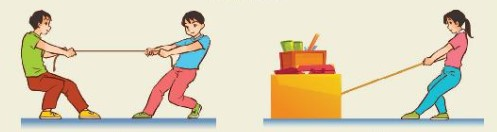
\includegraphics[scale=1]{../figs/VN10-2022-PH-TP019-3.jpg}
		\end{center}
	}
	
	\hideall
	{
		Xác định điểm đặt, phương, chiều của lực căng trong:
		
		- Hình a:
		
		+ Điểm đặt: tại 2 đầu sợi dây.
		
		+ Phương: trùng với phương của sợi dây.
		
		+ Chiều: ngược với chiều của lực do người kéo dãn dây.
		
		- Hình b:
		
		+ Điểm đặt: tại vật.
		
		+ Phương: trùng với phương của sợi dây.
		
		+ Chiều: ngược với chiều của lực do người kéo dãn dây.
		
	}
	\item \mkstar{3}
	
	{
		Lực kế trong hình đang chỉ ở vạch $\SI{10}{N}$.
		\begin{center}
			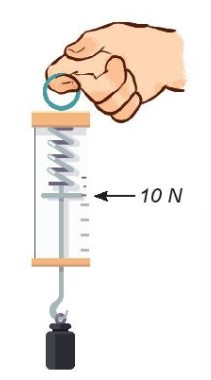
\includegraphics[scale=0.8]{../figs/VN10-2022-PH-TP019-1.jpg}
		\end{center}
		Tính trọng lượng và khối lượng của vật treo vào lực kế. Lấy $g \approx \SI{9,8}{m/s}^2$.
		
		
	}
	
	\hideall{
		
		Trọng lượng của vật là $\SI{10}{N}$. Khối lượng của vật là :
		
		$$m= \dfrac{P}{g} = \SI{1,02}{kg}.$$
		
		Vật chịu tác dụng bởi 2 lực cùng phương là lực hút trái đất có chiều từ trên xuống và lức kéo của lò xo có chiều từ dưới lên. 
		
	}
	
	\item \mkstar{3}
	
	
	{Đo trọng lượng của một vật ở một địa điểm trên Trái Đất có gia tốc rơi tự do là $\SI{9,8}{m/s}^2$, ta được $P = \SI{9,8}{N}$. Nếu đem vật này tới một địa điểm khác có gia tốc rơi tự do $\SI{9,78}{m/s}^2$ thì khối lượng và trọng lượng của nó đo được là bao nhiêu?
	}
	
	\hideall
	{
		Khối lượng của vật là
		
		$$ m = \dfrac{P}{g} = \SI{1}{kg}.$$
		
		Trọng lượng của vật ở nơi có gia tốc $\SI{9,78}{m/s}^2$ là
		
		$$P= mg = \SI{9,78}{N}.$$
	}
	\item \mkstar{3}
	
	
	{Một bóng đèn có khối lượng $\SI{500}{g}$ được treo thẳng đứng vào trần nhà bằng một sợi dây và đang ở trạng thái cân bằng.
		\begin{enumerate}[label=\alph*)]
			\item Biểu diễn các lực tác dụng lên bóng đèn.
			\item Tính độ lớn của lực căng. 
			\item Nếu dây treo chỉ chịu được một lực căng giới hạn $\SI{5,5}{N}$ thì nó có bị đứt không?
		\end{enumerate}
		
	}
	
	\hideall
	{
		\begin{enumerate}[label=\alph*)]
			\item Các lực tác dụng là: Lực hút của trái đất có chiều từ trên xuống và lực kéo của dây treo có chiều tư dưới lên, và chúng cùng phương.
			
			\item Độ lớn của lực căng dây 
			
			$$P= mg = \SI{4,9}{N}.$$
			
			\item 
			
			Nếu dây treo chỉ chịu được một lực căng giới hạn $\SI{5,5}{N}$, thì nó không bị đứt vì lực kéo của dây vẫn nhỏ hơn lực căng giới hạn.
		\end{enumerate}
	}
	\item \mkstar{3}
	
	
	{Một con khỉ biểu diễn xiếc treo mình cân bằng trên một sợi dây bằng một tay như hình. Hãy cho biết trong hai lực căng xuất hiện trên dây ($\vec T_1$ và $\vec T_2$), lực nào có cường độ lớn hơn? Tại sao?
		\begin{center}
			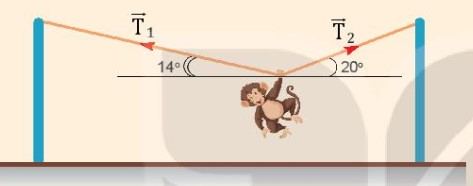
\includegraphics[scale=1]{../figs/VN10-2022-PH-TP019-2.jpg}
		\end{center}
	}
	
	\hideall
	{Con khỉ cân bằng:
		$$\overrightarrow{P}+\overrightarrow{T_1}+\overrightarrow{T_2}=\overrightarrow{0}$$
		Chiếu lên phương nằm ngang:
		$$T_1\cos\SI{14}{\degree}=T_2\cos\SI{20}{\degree}\Rightarrow T_1\approx0,97T_2$$
		Vậy $T_2>T_1$.
	}
	
	\item \mkstar{4}
	
	
	{
		Vật rắn $\SI{2}{kg}$ nằm cân bằng trên mặt phẳng nghiêng góc $30^\circ$. Lực căng dây có giá trị là bao nhiêu? Lấy $g=\SI{9,8}{m/s}^2$ và bỏ qua ma sát.
		\begin{center}
			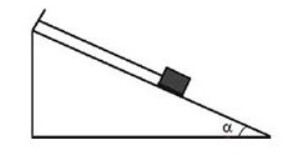
\includegraphics[scale=1]{../figs/VN10-2022-PH-TP019-5.jpg}
		\end{center}
	}
	
	\hideall
	{
		\begin{center}
			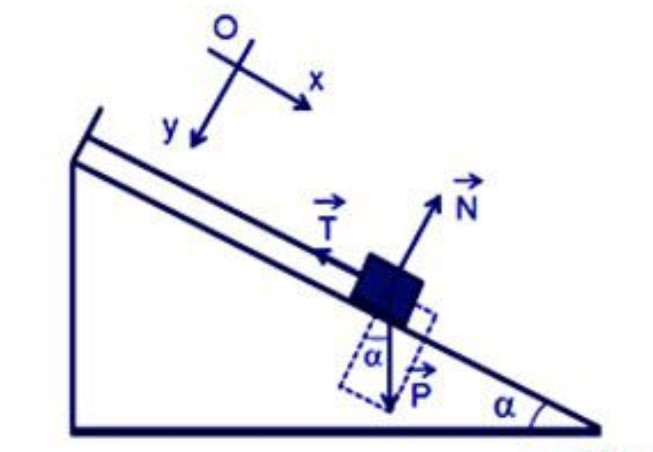
\includegraphics[scale=0.5]{../figs/VN10-2022-PH-TP019-4.jpg}
		\end{center}
		
		+ Các lực tác dụng lên vật gồm: trọng lực $P$, lực căng dây $T$, phản lực $N$.
		
		+ Ta có:
		
		$$\vec P + \vec T + \vec N = \vec 0\ (1).$$
		
		+ Gắn hệ trục tọa độ, chiếu (1) theo phương Ox, ta được:
		
		$$-T + P_\text{x} = 0 \Rightarrow T = P_\text{x} = P\sin \alpha = mg \sin \alpha = \SI{9,8}{N}.$$
		\textit{Có thể dùng tam giác vector để giải.}
		
	}
	\item \mkstar{4}
	
	
	{
		Một vật rắn khối lượng $\SI{5}{kg}$ được treo cân bằng trên mặt phẳng thẳng đứng bằng một sợi dây như hình vẽ. Bỏ qua ma sát, lấy $g=\SI{9,8}{m/s}^2$; $\alpha = 20^\circ$. Vậy lực căng dây là bao nhiêu?
		\begin{center}
			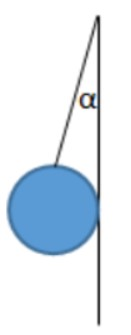
\includegraphics[scale=0.8]{../figs/VN10-2022-PH-TP019-6.jpg}
		\end{center}
	}
	
	\hideall
	{
		\begin{center}
			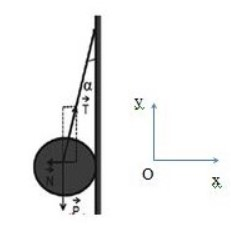
\includegraphics[scale=0.8]{../figs/VN10-2022-PH-TP019-7.jpg}
		\end{center}
		Các lực tác dụng lên vật gồm: trọng lực $P$, lực căng dây $T$ và phản lực $R$ của mặt phẳng thẳng đứng.
		
		Ta có:
		
		$$\vec P + \vec T + \vec N = \vec 0\ (1).$$
		
		Chọn hệ trục Oxy như hình, chiếu (1) theo các phương, ta được:
		
		$$ - P + T\cos \alpha = 0 \Rightarrow T = \dfrac{P}{\cos \alpha} = \SI{52,14}{N}.$$
	}
	\item \mkstar{4}
	
	
	{
		Treo một vật nặng khối lượng $\SI{6}{kg}$ vào điểm giữa của một sợi dây cáp căng ngang giữa hai cột thẳng đứng cách nhau $\SI{8}{m}$ làm dây võng xuống $\SI{0,5}{m}$. Lấy $g=\SI{10}{m/s}^2$. Tính lực căng của dây.
	}
	
	\hideall
	{
		\begin{center}
			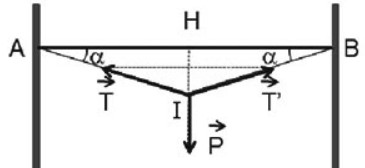
\includegraphics[scale=0.8]{../figs/VN10-2022-PH-TP019-10.jpg}
		\end{center}
		
		Theo đề bài ta có:
		
		$$T = T'; \text{IH} = \SI{0,5}{m}; \text{HA} = \SI{4}{m}.$$
		
		Vật cân bằng:
		
		$$\vec P + \vec T + \vec T' = \vec 0.$$
		
		Từ hình ta có:
		
		$$P = 2T \sin \alpha.$$
		
		Mặt khác, ta có:
		
		$$\tan \alpha = \dfrac{\text{IH}}{\text{HA}} = \dfrac{1}{8} \Rightarrow \sin \alpha = \text{0,124} \Rightarrow T = \dfrac{P}{2\sin \alpha} = \SI{241,9}{N}.$$
	}
	\item \mkstar{4}
	
	
	{
		Vật rắn nằm cân bằng như hình vẽ, góc hợp bởi lực căng của dây là $150^\circ$. Tính trọng lượng của vật biết độ lớn lực căng của hai dây là $\SI{200}{N}$.
		\begin{center}
			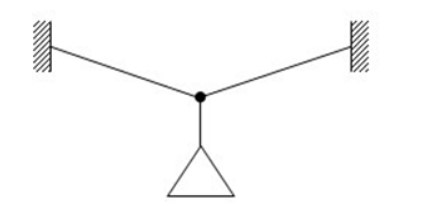
\includegraphics[scale=0.8]{../figs/VN10-2022-PH-TP019-8.jpg}
		\end{center}
	}
	
	\hideall
	{
		\begin{center}
			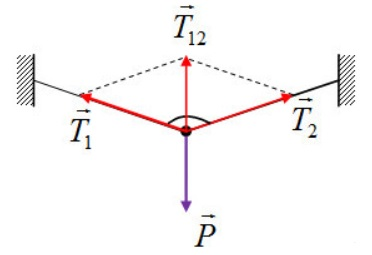
\includegraphics[scale=0.8]{../figs/VN10-2022-PH-TP019-9.jpg}
		\end{center}
		
		Ta có: 
		
		$$T_1 = T_2 = T = \SI{200}{N}.$$
		
		Vật nằm cân bằng nên:
		
		$$\vec T_1 + \vec T_2 + \vec P = \vec 0.$$
		
		Suy ra: 
		
		$$P = T_{12} = 2T \cos \dfrac{\alpha}{2} \approx \SI{103,5}{N}.$$
		
		
	}
	
	\item \mkstar{4}
	
	{ Một vật có trọng lượng $\SI{60}{\newton}$ được treo vào vòng nhẫn nhẹ O (coi là chất điểm). Vòng nhẫn được giữ bằng hai dây nhẹ OA và OB. Biết OA nằm ngang còn OB hợp với phương thẳng đứng góc $45^\circ$ (hình vẽ). Tìm lực căng của dây OA và OB.
		\begin{center}
			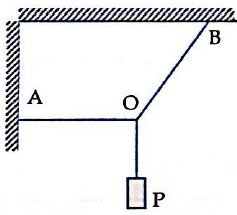
\includegraphics[scale=0.8]{../figs/VN10-2021-PH-TP011-1.jpg}
		\end{center}
	}
	\hideall{
		
		\begin{center}
			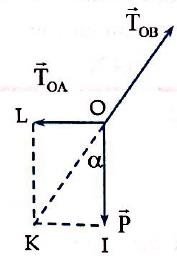
\includegraphics[scale=0.8]{../figs/VN10-2021-PH-TP011-2.jpg}
		\end{center}
		
		Các lực tác dụng vào điểm treo O như hình vẽ.
		
		Góc $\alpha$ là góc giữa OP và OB, $\alpha=45^\circ$.
		$$\text{OI}=\text{OK}\cdot \cos \alpha\Rightarrow \text{OK}=\dfrac{\text{OI}}{\cos \alpha}\Rightarrow T_\text{OB}=\dfrac{P}{\cos \alpha}=60\sqrt{2}\ \text{N} $$.
		
		Tương tự:   $$T_\text{OA}=T_\text{OB}\cdot \sin 45^\circ=60\ \text{N}$$
	}
\end{enumerate}